\documentclass[12pt,onecolumn]{article}
\usepackage{latexsym}
\usepackage{url}
\usepackage{float}
\usepackage{amsmath}
\usepackage{geometry}
\usepackage{subfig}
\geometry{left=2.0cm,right=2.0cm, top=2.0cm, bottom=2.0cm}
\usepackage{fancyhdr}
\usepackage{longtable}
\usepackage{url}
\usepackage{leftidx}
\usepackage{graphicx}
\usepackage{epstopdf}
\usepackage{subfig}
\usepackage{tikz}
\usepackage{ifthen}
%\usepackage{subcaption}
\usepackage{caption}
\newcommand\figref[1]{Figure \ref{#1}}
\linespread{1.5}
\author{Shuang Ao \\
Supervisor: Professor Charles Ling
}
\title{
\large\textbf{Unsupervised Feature Learning For Image Recognition}
}
\frenchspacing
\begin{document}
\maketitle
\tableofcontents
\newpage
\begin{abstract}
In image recognition, the success of machine learning algorithm is mainly depends on the image representation. Different representations can lead to different views of the image data. Although, the specific domain knowledge can help us for representation, sophisticate method for image representation is still crucial. In this TSP, firstly the background knowledge is introduced, including some basic feature extraction methods. Deep learning, which is introduced in Section 2, is the most popular method for feature extraction technique which has gained great reputations in both academic and industrial area. Finally, I present a novel method that is inspired by the idea of deep learning. In this method, I try to use patch combination as well as some ranking methods for image representation. The defects of this method can be my future work.

\end{abstract}

\section{Introduction to Image Filter}\label{sec:intro}
Image recognition is an important part in Computer Vision which includes many advanced machine learning techniques. A pattern recognition system (PRS) is an automatic system that aims at classifying the input pattern into a specific class\cite{kpalma2007overview}. An image recognition system
always proceeds in two steps: (1) generate several important features (descriptors or a book of code) (2) use a classifier
to distinguish the patterns with all these features. Compared to our human learning procedures, some prior knowledge should acquired
before the recognition which turns the learning procedure into be a supervised learning.

There are four major methodologies in image recognition:
\begin{itemize}
  \item Statistical approach. Here features are converted into a vector to present the pattern which can be a very easy to handle. This method
        is wildly and intensively used in practice.

  \item Syntactic approach. This method analysis the relationship between features and patterns are described in a hierarchical structure. For example
        (see \figref{sys}), the image on the right hand can be presented as the string ${d b a b c b a b d b a b c b a b}$.The system parses the set of extracted features using a kind of predefined grammar. If the whole features extracted from a pattern can be parsed to the grammar then the system has recognised the pattern. Unfortunately, grammar-based syntactic pattern recognition is generally very difficult to handle.

  \item Template matching. This can be the most intuitive way to localize and identify shapes in an image. Here, the method looks for the parts of the
        image which match the template. For each possible position in the image, it compares with each possible rotation or each possible geometric transformation of the template. According to certain metrics that can measure the similarity of these, the approach returns the most similar one. Since it has to compute all kinds of possibilities, this could be a very computational expensive approach.
  \item Neural networks. The an artificial neural network (ANN) had been used extensively before 2006 for image recognition. In 2006,  G. Hinton introduced "deep learning", a new method that can learning image features with fast unsupervised procedure which led to a revolutionary in image recognition\cite{hinton06}. We will
      discuss this method in details in section \ref{dl}.
\end{itemize}
\begin{figure}
  \centering
  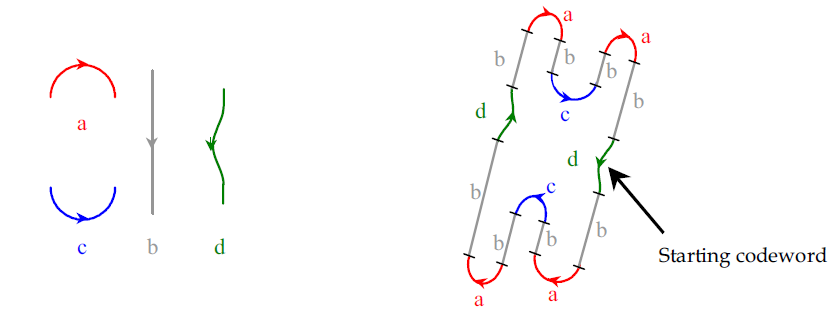
\includegraphics [width=6in] {fig/sys.png}\\
  \caption{Example of syntactic description features}\label{sys}
\end{figure}
There are some simple dependencies when representing the image patterns. One reason why explicitly dealing with image patterns is interesting is because they can be convenient to express many general priors about the world around us, i.e., priors that are not task specific but would be likely to be useful for a learning machine to solve AI tasks\cite{bengio2007scaling}. These general priors can sometime be used to help us design more powerful learners to discover the underlying factors that the data may reveal. Here are some examples of the general-purpose priors:
\begin{itemize}
  \item Smoothness: Assumes that the function $f$ to be learning for evaluation must satisfy that for any two patterns $x,y$, if $x\approx y, f(x)\approx f(y)$.
  %\item Multiple explanatory factors:
  \item A hierarchical organization of explanatory factors: Some patterns are more abstract than the others. These abstract patterns can be defined in terms of other patterns hierarchically.
  %\item Semi-supervised learning:
  %\item Shared factors across tasks
  %\item Manifolds:
  \item Natural clustering: Different values of categorical variables such as object classes are associated with separate manifolds. Humans have named categories and classes because of such statistical structure (discovered by their brain and propagated by their culture), and machine learning tasks often involve predicting such categorical variables.
 % \item Temporal and spatial coherence
  \item Sparsity: For any given observation $x$, only a small fraction of the possible factors are relevant\cite{olshausen1996emergence}. This means just a small fraction of the patterns can represent a image well.
  \item Simplicity of factor dependencies: The good abstract patterns can be related to each other through simple, typically linear combination.This can be seen in many neural networks when the top layer is just linear combination of the hidden units.
\end{itemize}







    \subsection{Kernel Based Method for Image Recognition}

No matter what classification techniques it is used, the images have to be transformed into certain kind of feature vectors with one of the
methodologies mentioned above. Image filter (also called \emph{kernel}) allows you to apply various effects on photos. In a 2D image, the 2D filter matrix \emph{f}
 can be applied with a convolutionary operation on the image \emph{I}:
\begin{equation}\label{eq:conv}
\left( {f * I} \right)\left( {x,y} \right) = \iint {f(x,y)I(x - t,y - t)dt}
\end{equation}

\begin{table}
  \centering
\begin{tabular}{|c| c| c|}
  \hline
  original & $\left[ {\begin{array}{ccc}  0&0&0 \\  0&1&0 \\  0&0&0\end{array}} \right] $ &\parbox[c]{5em}{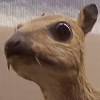
\includegraphics[scale=1.5]{fig/orig.png}}\\
  \hline
  edge detect & $\left[ {\begin{array}{ccc}  -1&-1&-1 \\  -1&8&-1 \\  -1&-1&-1\end{array}} \right] $ & \parbox[c]{5em}{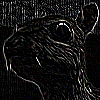
\includegraphics[scale=1.5]{fig/edge.png}}\\
  \hline
  blur & $\left[ {\begin{array}{ccc}  1&1&1 \\  1&1&1 \\  1&1&1 \end{array}} \right] $ & \parbox[c]{5em}{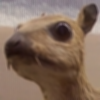
\includegraphics[scale=1.5]{fig/blur.png}}\\
  \hline
\end{tabular}
  \caption{Apply filters on image}\label{kl}
\end{table}

For a image classification task, the key issue is to find the most useful features to present the image. The results of the classification results can be greatly affected by the type of the kernels used. So there are two essential parts here: how to get the kernels and how to present the image with these kernels and the second part of the problem can be considered as the encoding the features. There are 3 different kernels defined in Table \ref{tab:edge}. After applying these kernels on the original image, the results are shown in the 3rd column. The size of the kernel can affect the image: the smaller the kernel is, it is more sensitive to some features in the image. However, the larger one is also useful while there are some noisy in the image as it is less possible to detect those tiny noisy pixels. From Furthermore there are many different kinds of kernels (with different properties and sizes) that can applied on the image to detect different features. For a specific problem, it is very difficult and inefficient to define any kernels even though we may acquire sufficient prior knowledge for this problem. And as the develop of the power of the computer and the complexity of the problem, it is not possible for one to get enough prior knowledge.
 \begin{figure}
  \centering
  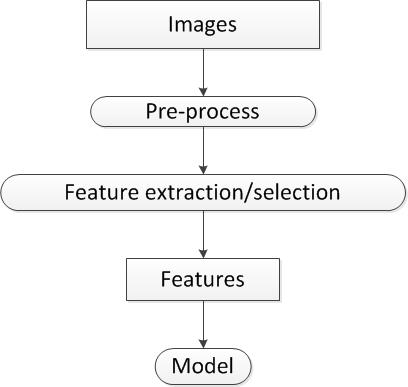
\includegraphics[scale=0.6]{fig/proces.jpg}\\
  \caption{Image Classification Procedure}
\end{figure}


\begin{table}
  \centering
  \begin{tabular}{cccc}
     \hline
     Original & Vertical Kernel 1 & Vertical Kernel 2 & Vertical Kernel 3\\
      \hline
      $\left[ {\begin{array}{ccc}  0&0&0 \\  0&1&0 \\  0&0&0\end{array}} \right] $
      & $\left[ {\begin{array}{ccc}  1&0&-1 \\  5&0&-5 \\  1&0&-1\end{array}} \right] $
      &$\left[ {\begin{array}{ccc}  -1&0&-1 \\  2&0&-2 \\  1&0&-1\end{array}} \right] $
      & $\left[ {\begin{array}{ccccc}   1     & 2     & 0     & -2    & -1 \\    4     & 8     & 0     & -8    & -4 \\    6     & 12    & 0     & -12   & -6 \\    4     & 8     & 0     & -8    & -4 \\    1     & 2     & 0     & -2    & -1 \\ \end{array}} \right]$\\
     \hline
     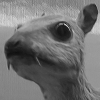
\includegraphics[scale=.5]{fig/gray.png} & 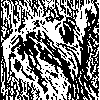
\includegraphics[scale=.5]{fig/v1.png}
     &  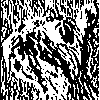
\includegraphics[scale=.5]{fig/v2.png}  &  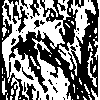
\includegraphics[scale=.5]{fig/v4.png}\\
     \hline
   \end{tabular}
  \caption{Different Kernels for Edge Detection}\label{tab:edge}
\end{table}

For a more heuristic way, many researchers try to learn the specific kernels for a particular task with either supervised or unsupervised learning strategies \cite{Berkes:2005}\cite{SVM99}\cite{hinton06}\cite{LeCun12}\cite{LeRMDCCDN12}. In kernel methods, the problem is modeled as a pairwise relation between data points which is captured in kernels. Thus, kernel functions (or simply kernels) have a profound impact on the performance of these learning algorithms \cite{AbbasnejadRR12}. However, tuning the kernels to fit the underlying hypotheses of the dataset can be a great challenge. As the images are taken in different situations, the light condition, the angle of the view and the shadow of the objects in the image would affect the performance of the kernels. On the other hand, mathematically kernel learning can be a constrained optimization task. Good kernels can map the images into high dimensional space which makes them more distinguishable. In an image recognition task, the image always includes at least thousands of pixels and there are also thousands of images for training. Optimization on these large high dimensional dataset, taking gradient descent for instance, can easily stuck into local minimum no matter how simple the objective function is. Also kernel learning can be considered as a problem similar to distance metric learning as the pixels in the image can be "activated" by a kernel if they are similar. But distance metric learning is trivial in image recognition which would be affected by many simple geometrical transformation such as rotation, shift or zoom in/out. In human brain, we do this unconsciously and parallelling. Many conventional distance metrics have been used in computer vision even though none these metrics can handle geometrical transformation. Thus before measuring the distance of the original image and the kernels, some transformations have to be apply on the original image such as rotation with different degrees (like from -30 degree to 30 degree with 1 degree interval), shift around (within a $9\times9$ window) and scaling in order to fit the kernel. Within these operations, maybe just one set of the combinations can have a high response which we couldn't know in advance. Yann LeCun \emph{et al} introduced \emph{ConvNet} which applies convolutionary operation on the whole image to learning the kernels\cite{Yann98}. Still ConvNet is one of the most popular methods with the best performance in real world image recognition\cite{CiresanIJCAI11}\cite{RanzatoNIPS06}\cite{KrizhevskyNIPS12}.

\begin{flushleft}
\emph{City Block Distance/Manhattan Distance}
\end{flushleft}
\begin{equation}
  d({P_1},{P_2}) = \sum\limits_{i = 1}^n {\left| {p_1^i - p_2^i} \right|}
\end{equation}

\begin{flushleft}
\emph{Euclidean Distance}
\end{flushleft}
\begin{equation}
  d({P_1},{P_2}) = \sqrt {\sum\limits_{i = 1}^n {{{\left( {p_1^i - p_2^i} \right)}^2}} }
\end{equation}

\begin{flushleft}
\emph{Cosine Distance}
\end{flushleft}
\begin{equation}
  d({P_1},{P_2}) = 1 - \frac{{{P_1}{P_2}^T}}{{\left\| {{P_1}} \right\|\times\left\| {{P_2}} \right\|}}
\end{equation}

As each image normally contains thousands of pixels, cutting the image into small patches can be a more realistic way when learning the kernels. 
\newpage
\section{Deep Learning Feature Representation}\label{dl}
     \begin{figure}[h]
  \centering
  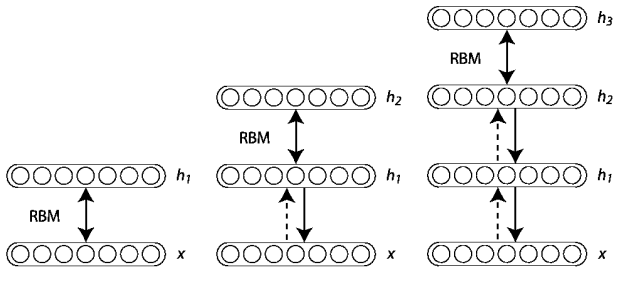
\includegraphics[scale = .5]{fig/dbn.png}\\
  \caption{Deep learning procedure}
\end{figure}
In 2006, a new feature learning and deep learning method was initiated by G.Hinton and has brought great impact in both academic and industrial field. This deep learning method is a kind of deep neural network which contains several layers. The core idea, referred to as \emph{greedy layerwise unsupervised pretraining} was to learn the bottom to top hierarchical features in a deep neural network. In deep learning, each layer is trained separately which makes is really fast and the output of the lower layer is the input of the higher one. When using greedy layerwise unsupervised pretraining, the two conjunctival layers can regarded as a Restrict Boltzman Machine (RBM) and the \emph{Energy} of the RBM is defined as\cite{Hinton12}:
\begin{equation}\label{eq:engery}
  E(v,h) =  - \sum\limits_{i \in visible} {{a_i}{v_i}}  - \sum\limits_{j \in hidden} {{b_j}{h_j}}  - \sum\limits_{i,j} {{v_i}{h_i}{w_{ij}}}
\end{equation}
Here, $v_i$, $h_j$ are the visible value (input) and the hidden value (output) respectively, and $a_i$, $b_j$ are their bias . $w_{ij}$ is the weight of the visible node $i$ and hidden node $j$. The probability that the RBM can recall the visible vector, $v$, is defined as:
\begin{equation}
\begin{gathered}
  p(v) = \frac{1}{Z}\sum\limits_h {{e^{ - E(v,h)}}} \\
   Z = \sum\limits_{i,h} {{e^{ - E(v,h)}}}  \\
\end{gathered}
\end{equation}
The derivative of the log probability of a training vector with respect to a weight is:
\begin{equation}
\begin{gathered}
  \frac{{\delta \log p(v)}}{{\delta {w_{ij}}}} = {\left\langle {{v_i}{h_j}} \right\rangle _{data}} - {\left\langle {{v_i}{h_j}} \right\rangle _{model}}\\
  {\left\langle {{v_i}{h_j}} \right\rangle _{model}} \approx {\left\langle {{v_i}{h_j}} \right\rangle _{recon}}\\
  \end{gathered}
\end{equation}\label{eq:weight}

\begin{figure}[h]
\centering
\def\layersep{1.5cm} % Gap between visible & hidden units
\def\numvis{3} % Number if visible units
\def\numhid{4} % Number of hidden units
\begin{tikzpicture}[
    node distance=\layersep,
    line/.style={<->,shorten >=2pt,shorten <=2pt,>=stealth}
    ]
    \tikzstyle{neuron}=[circle,fill=black!25,minimum size=21pt,inner sep=0pt];
    \tikzstyle{visible neuron}=[neuron, fill=green!50];
    \tikzstyle{hidden neuron}=[neuron, fill=orange!75];
    \tikzstyle{annot}=[text width=4em];

    % Iterate over visible units
    \foreach \name / \y in {1,...,\numvis}
        \node[visible neuron] (V\name) at (\y,0) {$v_\y$};

    % Iterate over hidden units
    \foreach \name / \y in {1,...,\numhid}
        % Calculate the appropriate offset for the hidden unit based on the
        % number of visible units.
        \pgfmathparse{\y + (\numvis - \numhid) * 0.5}
        \node[hidden neuron] (H\name) at (\pgfmathresult, \layersep) {$h_\y$};

    % Draw a double-arrow connector between the each unit
    \foreach \source in {1,...,\numvis}
        \foreach \dest in {1,...,\numhid}
            \draw[line] (V\source) -- (H\dest);

    % use if/then/else to decide where to draw the labels
    \ifthenelse{\numvis > \numhid}
    {
        \node[annot,left of=V1, node distance=1cm] (hl) {Visible};
        \node[annot,above of=hl] {Hidden};
    }
    {
        \node[annot,left of=H1, node distance=1cm] (hl) {Hidden};
        \node[annot,below of=hl] {Visible};
    }
\end{tikzpicture}
\label{fig:rbmtopology}
\caption[RBM Topology]{Restricted Boltzmann topology with \numvis{} visible units and \numhid{} hidden units.}
\end{figure}

Even though,  the ${\left\langle {{v_i}{h_j}} \right\rangle _{model}}$ can't be calculated, Hinton proposed a fast learning procedure, called \emph{Contrastive Divergence}, that can estimate it by ignoring the tricky term in the objective function and proved that this can lead to the convergence. Sutskever and Tieleman have shown that this procedure is not following the gradient of any function\cite{SutskeverT10}.
\begin{figure}
  \centering
  % Requires \usepackage{graphicx}
  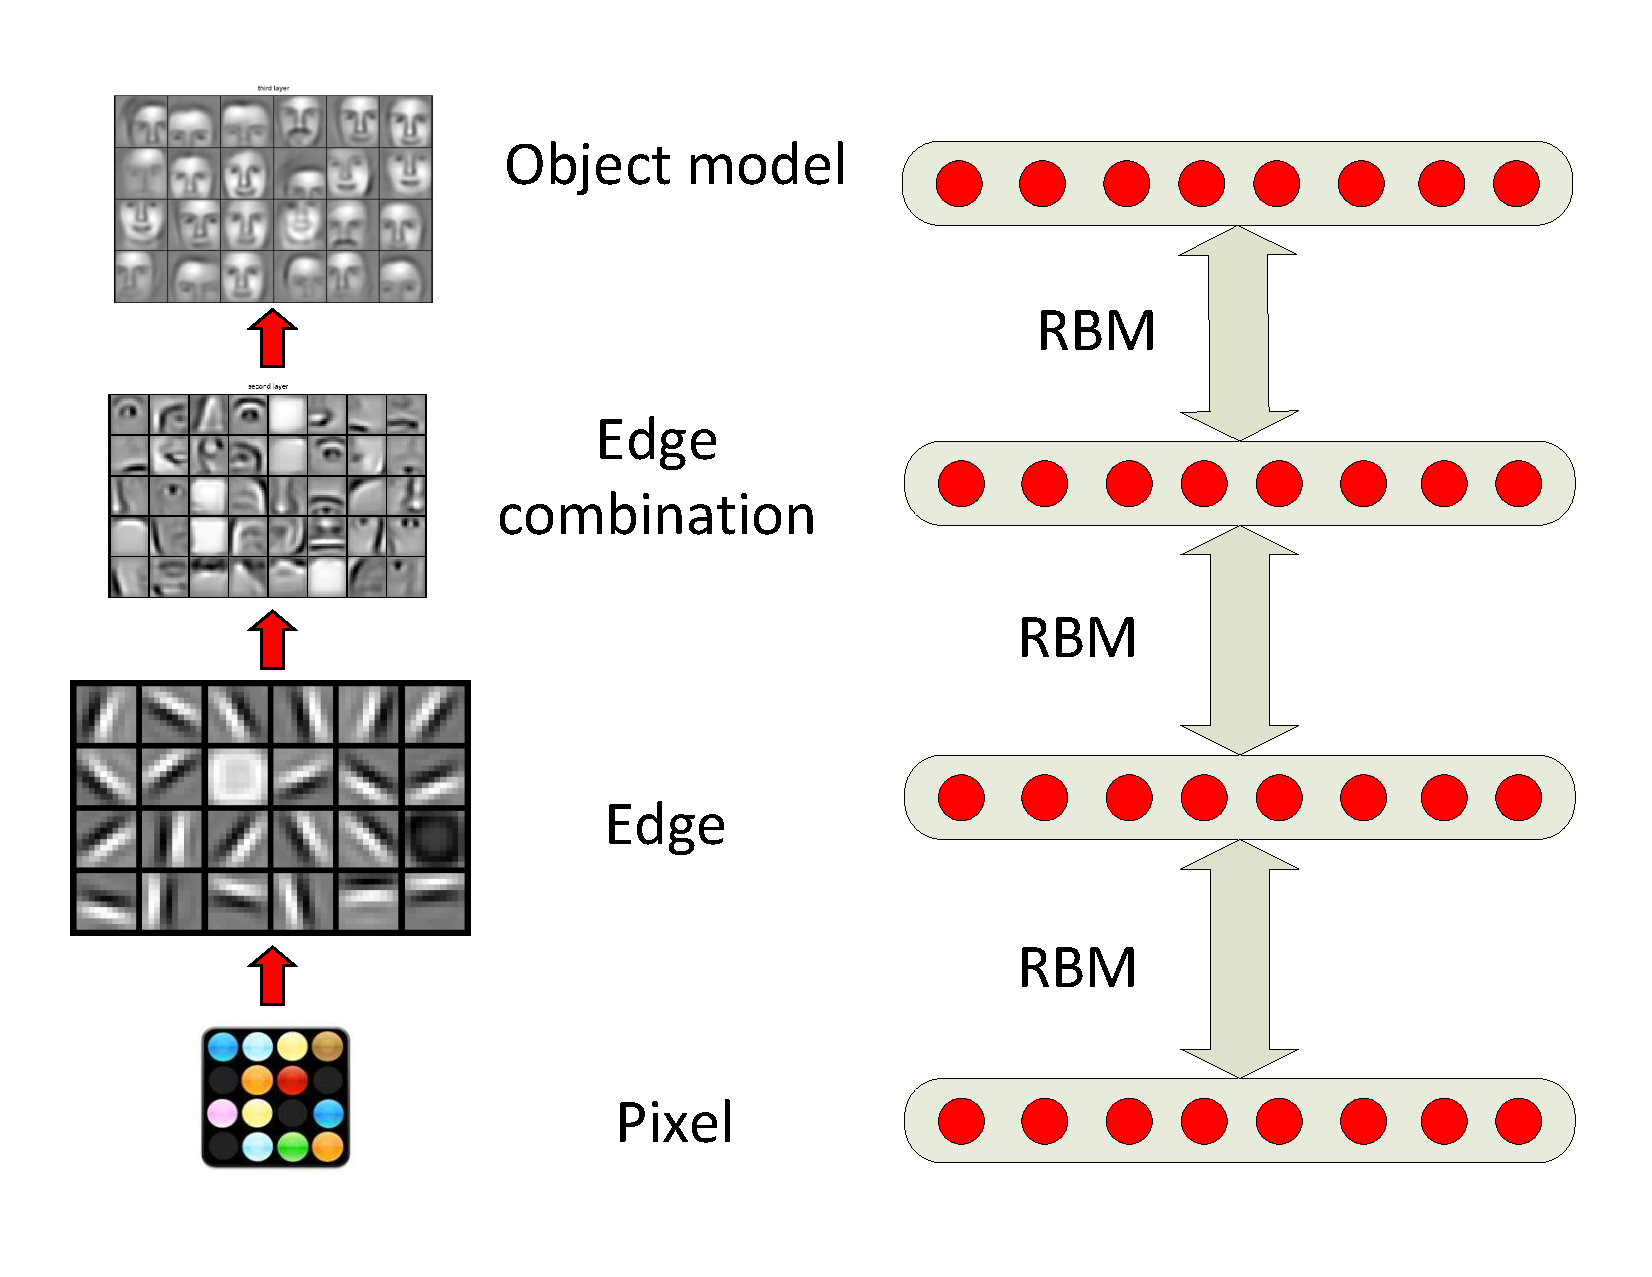
\includegraphics[scale=.5]{fig/deeplearning.pdf}\\
  \caption{Hierarchical Representation of Deep Learning}
\end{figure}

After this greedy layerwised unsupervised pretraining, the configuration of the deep network can be the initial of the supervised deep neural network predictor\cite{Srivastava13}. And the stochastic gradient descent can be applied for further optimization. The initial configuration after greedy layerwised unsupervised pretraining can make this deep network get rid of the local minimum since the supervised procedure is not based on any gradient method.

It is interesting to ask why this greedy layerwise unsupervised pretraining can help in supervised learning\cite{ErhanCBV10}. The curriculum greedy layerwise unsupervised pretraining tries to build some intermediate representations rather than some distinguishable representations. This is nicely related to curriculum learning idea which indicates that it is much more easier to learn some simpler concept first and build a much more complicated ones on top of the simpler ones\cite{BengioICML09}. For a deep supervised classifier, in the unsupervised training procedure, the deep neural network is the stacked RBMs which can initialize in a \emph{good} local minimum where the \emph{good} refers to low generalization error\cite{Bengio13}.

Stacked RBMs has been developed for many large learning problems as the feature extractor for other supervised classifiers. In these cases, stacked RBM is used as both feature extractor to learn the hierarchical representations and autoencoder to evaluate the similarity between the features and the images.  However, single-layer RBM can still be a good predictor for a supervised learning problems. H.Larochelle used the RBM stand-alone to build the discriminative RBM on character recognition without replying on any other classifier\cite{LarochelleB08}. Even though, for the large learning task, deep neural network with millions or even billions of nodes can get some good results\cite{krizhevsky2012imagenet}\cite{LeRMDCCDN12}, in some simple shadow network can still do well. It's a big waste to use a cannon to kill a mosquito.

When training the deep neural network, there are many details that can speed the convergency of the stacked RBMs to achieve a better local minimum. Cho et al. proposed a adaptive learning rate for the RBM training as well as a novel gradient estimator that takes into account the invariance of the model to flipping hidden unit bits and inverting signs of corresponding weight vectors\cite{cho2011}.  For the choice of the hidden units, several experiments have shown that nonlinearity could influence both training and generalization performance\cite{GlorotB10}\cite{GlorotBB11}\cite{NairH10}. Moreover, the initial weights can affect the training results. A good initialization can substantially reduce the difficulty of training the deep neural network. With a sparse initialization or using often saturated nonlinearities, it is more promising to make the hidden units specialized\cite{martens2010deep}. For the training method, there is still a debate between online learning method such as stochastic gradient descent and using large mini batch(thousands of samples)\cite{LeNCLPN11},  even though, the stochastic gradient descent and its invariants are more popular and have won many competitions. As we can see in Equation (\ref{eq:weight}), most of the computation in updating the weights can be done with matrix operations, it is more convenient to use GPU to do these jobs which is designed to accelerate the matrix operations\cite{raina2009large}. Normally, training the huge deep network on GPU can be at least 10 times faster than training on CPU.

Despite great achievement in both academic and industrial area, there are still some criticisms, one of which is that there are so many hyperparameters and variants that exploring the configuration and the architecture is really an art\cite{LeCunBOM12}. To solve this problem, many automating hyperparameters searching works have been proposed recently which makes it more convenient and efficient\cite{BergstraB12}\cite{BergstraBBK11}\cite{snoek2012practical}. To deal with large quantities of image recognition problem, deep learning can be the first choice. As a neural network, it can easily get rid of the local  minimum, which is the biggest issue in all the large neural network training procedure, with just a little prior knowledge through the efficient unsupervised training. However, recent work on large quantities of labeled data shows that with a proper initialization, the pure deep supervised network can still be successfully trained without any layerwised pre-training\cite{cirecsan2010deep}\cite{glorot2011deep}\cite{seide2011conversational}. And in this situation, the layerwised unsupervised pretraining can bring little or even no improvement over the supervised one when training for long enough.

In addition, deep learning will be the most promising method for image recognition in the next few years. Even though pure supervised learning can compete with deep learning while there are enough labeled data for training, still deep learning and unsupervised pre-training for image recognition would be the future. As in real world, we can always obtain enough data while just a very small fraction can be labeled. Unsupervised feature extraction techniques can be a more realistic method. 


 \newpage
\section{K-means Feature Representation}\label{km}
    Deep neural network has shown its great power on large scale image recognition tasks, but sometimes it is more important to get good representation of the image rather than learning the complex hierarchical representations\cite{CoatesNL11}. The main drawback of learning the high-level representation for many systems is their complexity and expense. Moreover, the multi hyper-parameters of these algorithms which would affect the performance significantly require many prior knowledge as well as computational expensive validation to determine their values. Since the unsupervised pre-training can learn some important representations,  as one of the most basic and fast unsupervised learning strategy, K-Means can also learn the representation well through a self-taught procedure. For a K-Means algorithm, the only parameter $K$ decides the number of the centroids that the data can generate. As a mature algorithms, there are many techniques that can accelerate its convergence\cite{pelleg1999accelerating}\cite{pelleg2000x}\cite{gibou2002fast}. K-Means has been defined as a successful method to learn features
from images by computer vision researchers. The term of "bag of features" is very popular in computer vision communities\cite{csurka2004visual}\cite{lazebnik2006beyond}.

In our system, the feature representation is learned as the following steps:
\begin{enumerate}
  \item learning the bag of features from sub-patches with K-Means to get a low level features.
  \item combining the low level features to generate a higher-level features.
  \item mapping the image to the feature space and do the classification.
\end{enumerate}
The concept of an ROIs (region of interests) is commonly used in many application areas especially in medical image (magnetic resonance imaging, MRI) process\cite{desikan2006automated}. It is based on a simple and intuitive hypothesis: there could always be some objects or features that appear in some certain location of the image which can be used to identify the image. This hypothesis can be applied to many other real world applications such as hand digital recognitions.
\begin{figure}
  \centering
  % Requires \usepackage{graphicx}
  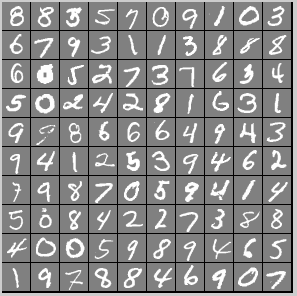
\includegraphics[scale = 1]{fig/MNST.png}\\
  \caption{The first 100 images in MNST dataset}
\end{figure}

\subsection{learning the patches with K-Means}
The classic K-means clustering algorithm finds cluster centroids that minimize the distance between data points and the nearest centroid.Also called
"vector quantization", K-means can be viewed as a way of constructing a dictionary $D \in {R^{n \times k}}$ of k vectors so that a data vector $x_(i) in R_n, i = 1...;m$
can be mapped to a code vector that minimizes the error in reconstruction.
\begin{equation}\label{}
  \mathop {\min }\limits_S {\text{ }}\sum\limits_i ^k{\sum\limits_{{x_j} \in {S_i}} {{{\left\| {{x_j} - {\mu _i}} \right\|}^2}} }
\end{equation}
$\mu_i$  is the mean of $S_i$.

In our task, the images are $28 \times 28$ pixels grayscale images and we use $14 \times 14$ pixels patch presented as a 196 pixel intensities for the K-means to learn the features. We select 12 location to generate the patches (shown in \figref{location}). For each location we use K-means to get 100 centroids with \emph{K-means++} which can avoid the sometimes poor clusterings found by the standard k-means algorithm.\cite{arthur2007k}.
\begin{figure}
  \centering
  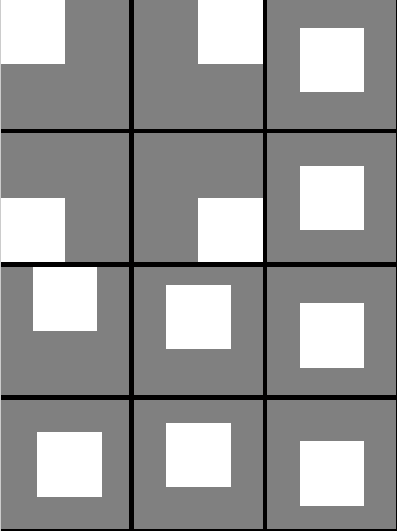
\includegraphics[scale=.5]{fig/patch_location.png}\\
  \caption{The 12 locations of the patch}
\end{figure}\label{location}

\begin{figure}[t]
  \centering
  \subfloat[Location of the patch in original image]{
  \raisebox{15mm}
    {
\includegraphics[scale=.8]{fig/patch1.png}}
  }
  \qquad
  \subfloat[100 Centroids of this location]{
     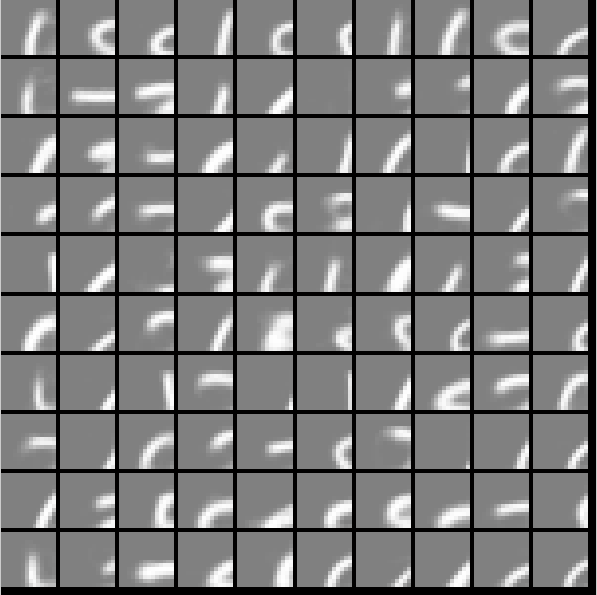
\includegraphics[scale=.5]{fig/c1.png}
  }
  \caption{The Centroids for location 1.}
\end{figure}


\subsection{Patch Combination}
The initial intuition of patch combination is the hierarchical feature representation. The higher level features can be presented as the combination of the lower ones. The idea of sparse coding is also to use the lower level features to represent the higher ones with linear combination\cite{GrosseRKN07}. In sparse coding, the lower features are linearly overlapped on each other to generate the complex higher level ones and the dimensions of the new feature will never change. In our task,  we don't overlap the lower ones. Alternatively, as we already know the specific location of each patch in the original image, we can combine the lower features in different locations of the image and generate the higher ones.
\begin{figure}[h]
  \centering
  % Requires \usepackage{graphicx}
  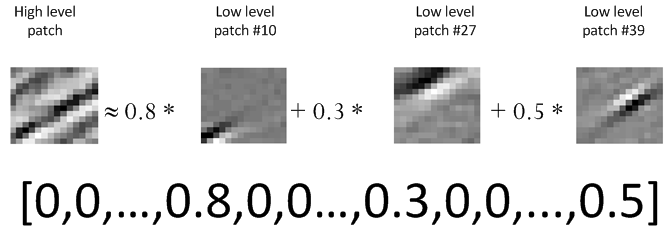
\includegraphics[scale = .75]{fig/sparsecoding.png}\\
  \caption{The idea of sparse coding}
\end{figure}
\begin{figure}[h]
  \centering
  % Requires \usepackage{graphicx}
  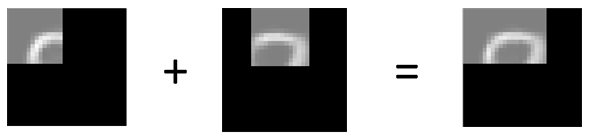
\includegraphics[scale = .75]{fig/patchcombine.png}\\\
  \caption{The combination of patches in different locations of the image}
\end{figure}
When combining two low level features, the most simple method could be just consider the number of the common instances that appear in both. If they have a lot of instances in common, these two low level features can be combined as a new one. Consider the image dataset $D$ has $n$ instances $(D \in R^{n \times m})$ and for each candidate patch location $l$ which are clustered into $k$ clusters, $D$ can be represented as a sparse binary matrix $D^l \in R^{n \times k}$
\begin{equation}
  D^l _{i,j}= \left\{ \begin{gathered}
  {D^l_{i,j}} = 1,{\text{ if }}{D_i} \in {\text{cluster }}j \hfill \\
  {D^l_{i,j}} = 0,{\text{ if }}{D_i} \notin {\text{cluster }}j \hfill \\
\end{gathered}  \right.
\end{equation}
When we have two patch location candidates $l_1$ and $l_2$, $C^{com}=D^{l_1} \times {D^{l_2}}^T$ and $C^{com}_{i,j}$ denotes the number of the common instances that for $i_{th}$ cluster in $l_1$ and $j_{th}$ cluster in $l_2$. However, $C^{com}$ just indicates how many instances that both of these two clusters hit but ignores the how many instances actually there are in each of the clusters. For instance, cluster A and cluster B has 100 and 200 instances respectively and $C^{com}_{A,B}=100$, if cluster C and cluster D has 1000 and 800 instances respectively and $C^{com}_{C,D}=150$, it is hard to say that the combination of C and D is better than A and B.

Alternatively, to evaluate the quality of the combination of the $k_1$ cluster in $l_1$ and the $k_2$ cluster in $l_2$, we can get the $k_1$ and $k_2$ column of the sparse matrix $D^{l_1}$ and $D^{l_2}$ and get the confusion matrix as Table \ref{confusion}. In the method we mentioned above, the \# of instance in common just take the \emph{True Positive} into account while ignoring the impact of \emph{False Positive} and \emph{False Negative}. In pattern recognition, the concept of \emph{precision} and \emph{recall} which are defined as Equation (\ref{eq:pr}),can solve this problem\cite{powers2011evaluation}. From Table \ref{confusion}, the precision and recall are switched when we switch cluster $i$ and $j$. But we want some score which can satisfy $score(i,j) = score(j,i)$.
Here precision and recall refer to the fraction of the "hit" in both clusters. And \emph{F-measure} can take both recall and precision into account which is defined as Equation(\ref{eq:fm}). If we set $\beta = 1$, $F_1$ is symmetric for precision and recall. So we can get $F_1(i,j) = F_1(j,i)$. For each pair of location candidates $l_1$ and $l_2$, each of which consists of $k$ centroids, we can get a $k \times k$ symmetric matrix $ComScore=\left\{ComScore_{i,j}|ComScore_{i,j}=F_1(i,j),i,j=1,2,...,k \right\}$ where $ComScore_{i,j}$ indicates the F-measure for the combination of $i_{th}$ cluster in $l_1$ and the $j_{th}$ cluster in $l_2$. If $ComScore_{i,j}$ is great than some threshold $\theta$, then the new location $l_1+l_2$ will include the centroid $k_1+k_2$ and the membership of the new centriod would be the instances in both of these two clusters.
\begin{equation}\label{eq:pr}
  \begin{gathered}
  precision = \frac{{TP}}{{TP + FP}} \hfill \\
  recall = \frac{{TP}}{{TP + FN}} \hfill \\
\end{gathered}
\end{equation}

\begin{equation}\label{eq:fm}
 {F_\beta } = \left( {1 + {\beta ^2}} \right)\frac{{precision \cdot recall}}{{\left( {{\beta ^2} \cdot precision} \right) + recall}}
\end{equation}
\begin{table}[H]
  \centering
  \begin{tabular}{ |l | p{5cm}| p{5cm}|}
  \hline
    & j & $\neg$ j \\
    \hline
  i& \# of instances both has $i_{th}$ and $ j_{th}$ feature (True Positive)& \# of instances only has $i_{th}$ feature (False Positive)\\
   \hline
  $\neg$ i & \# of instances only has $j_{th}$ feature (False Negative) & \# of instances has neither $i_{th}$ nor $ j_{th}$ feature (True Negative)\\
  \hline
\end{tabular}
  \caption{Confusion Matrix for cluster $i$ and cluster $j$}\label{confusion}
\end{table}
From \figref{fig:comb} we can see that, the combination of the patch location are very flexible, which can create some ambiguous shapes of patches that can describe some important features in the image. Compared with the conventional convolutionary method, which requires large computing and is very sensitive to the size of the kernels, our method can generate kernels with any size and any shape from some small lower patches.
\begin{figure}[h]
 \centering
\begin{tabular}{c}
   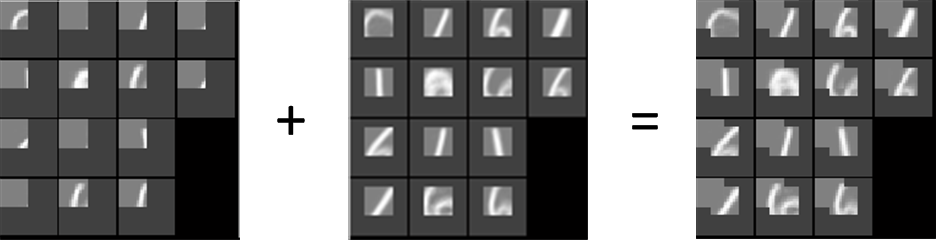
\includegraphics[scale = .5]{fig/combine2.png}\\
   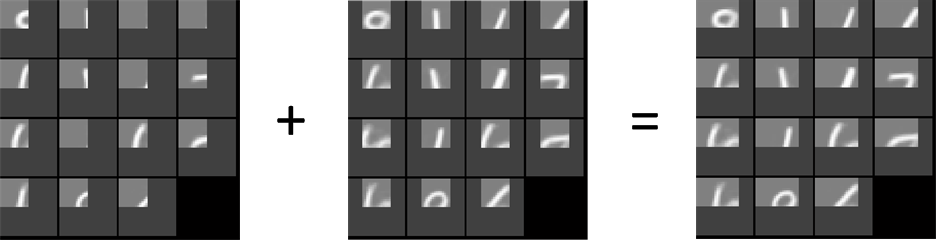
\includegraphics[scale = .5]{fig/combine.png}\\
\end{tabular}
  \caption{Successfully combined patches}\label{fig:comb}
\end{figure}

\subsection{Patch Ranking}

From the patch combination, for a particular threshold $\theta$, we can get many features with ambiguous size and shape. These centroids, generated from either k-means (low level features) or combination of the lower feature(high level features), are used as the template for the image representation. But too many features can lead the algorithm to be very slow as well as some duplicate features. Therefore, some less informative centroids (templates) should be removed. These centroids should be redundant, duplicate or irrelevant. Here both the supervised and unsupervised patch ranking techniques can be used. Unsupervised patch ranking is used to eliminate the centroids whose clusters are either too sparse or too small. Supervised patch ranking is used to eliminate those centroids that are duplicate which can no longer provide extra information after the class label is introduced.

\begin{figure}[t]
  \centering
  \subfloat[Clusters with the same centroids but different $\mu$]{   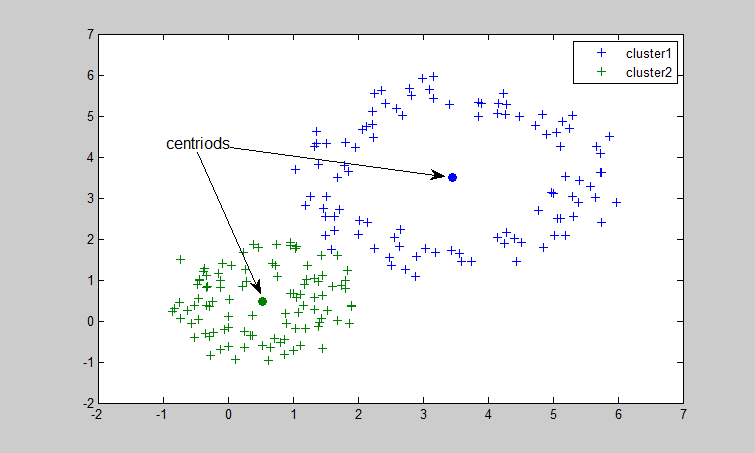
\includegraphics[scale = .5]{fig/cluster_cmp1.png}}
  \\
   \subfloat[Clusters with the almost the same centroids but different size]{ \label{fig:cmp2}  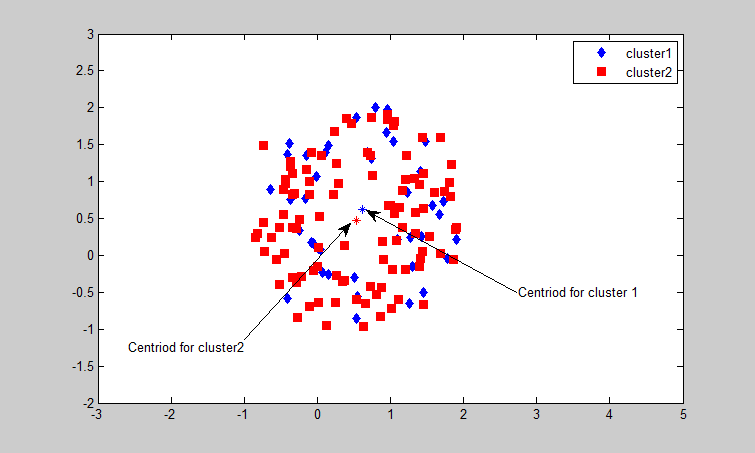
\includegraphics[scale = .5]{fig/cluster_cmp2.png}}
  \caption{Two situation to evaluate the cluster/centroid}
\end{figure}
\subsubsection{Unsupervised Patch Ranking}

In all these centroids we get from patch combination , some of the lower ones would be less informative after they are successfully combined to generate the higher ones. For instance, if $k_1$ centroid in $l_1$ and  $k_2$ centroid in $l_2$ have identical membership in the original image set and they can definitely generate a higher centroid $k_3$ in location $l_3$ which will contain identical membership as $k_1$ and $k_2$. In this situation,  $k_1$ and $k_2$ would be the duplicate patches as the higher level centroid $k_3$ can provide the information as much as them. However, we can not simply assume that all the lower features are less informative than the higher ones. Normally lower clusters can have more instances belong to compared with higher ones.In \figref{fig:cmp2}, cluster 1 has 40 instances while cluster 2 has 100 instances. The distance of them are very near and they all have the almost the same average distances to the centroid. Here, the cluster 2 is more general and its centroid can better describe the feature of its member. A more complicated situation could be the comparison of the centroids with different shape. Here we introduce the following equation for evaluation of the centroid.
\begin{equation}\label{eq:rank}
  Dist(x,C) = \underbrace {\frac{1}{n}\sum\limits_{i = 1,{x_i} \in C}^n {\frac{{{x_i} \times C}}{{\left| {{x_i}} \right|\left| C \right|}}} }_{mean{\text{ cosine similarity}}} + \alpha  \cdot  \underbrace {\log \left( n \right)*\log ({C_{size}})}_{\begin{subarray}{c}
  {\text{size of the cluster and }} \\
  {\text{size of the centroid}}
\end{subarray} }
\end{equation}
Here, the $x$ is all the cluster members and $C$ is their centroid. $n$ denotes the size of the cluster and the $C_{size}$ is the size of the number of pixels of the centroid $C$ which is positive proportional to the level of the feature. The first part of Equation (\ref{eq:rank}) is the mean cosine distance of the cluster members to the centroid which describe the similarity among the cluster members. Cosine Similarity is to calculate the orientation of two vectors instead of the magnitude which is less sensitive to the size of the pixels evaluating the centroids with different number of pixels.
The second part is for normalization which involves the size of the cluster and the size of the centroid. Our intuition is that if two clusters have the same similarity among their members, the higher level feature/centroid and the cluster with more instances has a higher rank.

Even though, there are many mature techniques for cluster analysis (like Davies–Bouldin index\cite{davies1979cluster}, Dunn index\cite{dunn1973fuzzy}, etc), which is the essence method to obtain the templates,we still want to use the most basic criterion, mean distance to the centroid, as our fundamental criterion. The unsupervised ranking is used here as the prior method of the supervised one which can be more sophisticate and useful than the unsupervised one. And it is better to use to unsupervised ranking before the supervised one as there could be too centroids, if we can't eliminate some of them with the fast unsupervised one, it could be very slow for the supervised ranking method to deal with a lot of centroids.

\subsubsection{Supervised Patch Ranking}
After eliminating the sparse centroids, the supervised patch ranking can eliminate more duplicate and irrelevant centriods to improve the results. This procedure can be considered as the feature selection which is very important in the pattern recognition system. Our ultimate goal is to improve the classification result after the patch ranking. However, without supervised ranking, there could be some embarrassing situations, like in \figref{fig:unsup_100}. For the classification of digital number 1 and 3, some important features for both of the classes should be found before the final classification. But after the unsupervised ranking, most of the features with higher rank are for the digital 1. There is just one feature (in red box) for digital 3. Even though this matters a little for the binary situation, this could be a serious problem for multi-class problem as some of the classes may not get enough features to be distinguished. So the goal of the supervised ranking is to found those centroids that can represent each of the classes and eliminate the redundant and irrelevant ones.
\begin{figure}[H]
  \centering
  % Requires \usepackage{graphicx}
  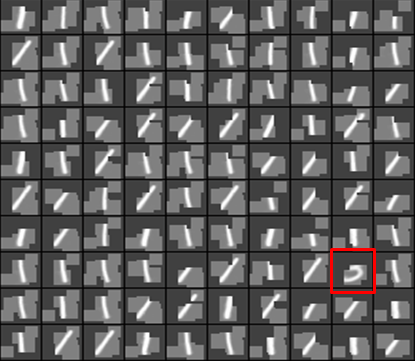
\includegraphics[scale = .5]{fig/100_unsup.png}\\
  \caption{Top 100 unsupervised ranking centroids for classification of digital number 1 and 3}\label{fig:unsup_100}
\end{figure}
\textbf{Significant Test}
The typical supervised feature selection can be formulated like: given the dataset $D$ that contains $N$ samples with $M$ features $F={f_i, i=1,...,M}$ as well as the target class $c$, feature selection is to find the optimal subspace $m$ of the $M-dimension$ that can best characterized $c$. As there could be $2^M$ candidates, it is really hard to search the space exhaustively. Here the $optimal$ leads to the $minimal classification error$ which is to find the maximal statistical dependency of the target class $c$ on the data distribution in the subspace $R^m$.  From this, the most simple method could be the significant test for each feature with specific target class $c$.
\begin{figure}[H]
  \centering
  % Requires \usepackage{graphicx}
  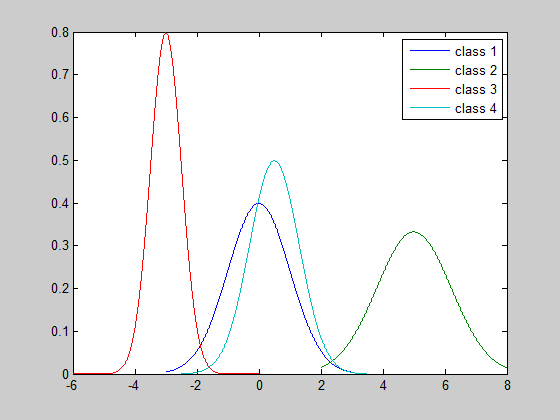
\includegraphics[scale = .75]{fig/sign.png}\\
  \caption{Significant test for feature selection for the 4 classes situation for specific feature $f_i$}\label{fig:sign}
\end{figure}
From \figref{fig:sign} it is easy to find that the class 1 and class 4 are almost overlapped and with some significant test (like $t-test$), class 1 and class 4 can not be distinguished with the feature $f_i$. Still, there should be some criterion for the supervised ranking with significant test:
\begin{enumerate}
  \item Features that are significantly distinguishable for all classes should be rank the highest. These features are global features that can be used to "vote accept" for the every class.
  \item Features that are significantly distinguishable for more classes should be rank higher. These features are local feature for specific one or more classes and they can "vote reject" for at least one class.
  \item Features that are not significantly distinguishable for all classes are the redundant and irrelevant ones which should be eliminated and rank the lowest.
\end{enumerate}

\textbf{Mutual Information}
The significant test can check the dependency of target class on the data distribution for some features. It is easy to check for a single feature, as we want to find the best $m$ features and the final performance is determined by the joint result of the features, the significant test can't solve this well. In information theory, the mutual information of two random variables is a measure of the mutual dependence of the two random variables. Given two random variables $X$ and $Y$, their mutual information is defined in terms of their probabilistic density functions $p(x)$, $p(y)$, and $p(x,y)$:
\begin{equation}\label{mutualinfor}
  I(X,Y) = \int_Y {\int_X {p(x,y)\log \frac{{p(x,y)}}{{p(x)p(y)}}dx} dy}
\end{equation}
Intuitively, mutual information measures the information that X and Y share: it measures how much knowing one of these variables reduces uncertainty about the other. For example, if X and Y are independent, then knowing X does not give any information about Y and vice versa, so their mutual information is zero. At the other extreme, if X and Y are identical then all information conveyed by X is shared with Y: knowing X determines the value of Y and vice versa. As a result, in the case of identity the mutual information is the same as the uncertainty contained in Y (or X) alone, namely the entropy of Y (or X: clearly if X and Y are identical they have equal entropy) \cite{mackay2003information}. Here Y can be the target class $c$ and X can be any dimension (feature) in the $M-dimension$ space. For each individual feature, $I(X,c)$ reflects the dependency of the class on the feature X. the top $m$ $I(X,c)$ in descending order are the features to be selected.

It is clear that in neither significant test nor mutual information criterion, the top $m$ selected features are not necessarily to be the "$m$ best features" as the relationship between the features is not considered. To obtain the "$m$ best features", it is to search the best $m$ combination of the features which can be applied in two opposite directions with the filter: forward  and the backward selections \cite{peng2005feature}.
\begin{enumerate}
  \item The forward selection tries to select a subset of $m$ features from $M$ in an incremental way. At first we set the candidate set $S_{cand}=M$ and $S_{sel} = \emptyset$ as well as the criterion for the selection $Cr$. For each iteration, we pick up a feature $x$ from $S_{cand}$ and evaluate $Cr(x+S_{sel})$. The best $x_{best}$ will be add into $S_{sel}$ as well as remove from $S_{cand}$. This would stop in $m$ iterations.
  \item The backward selection manners from the other direction. It first set $S_{sel} = M$ and subtract the irrelevant features from it until stop. The backward selection is often used to select a large subset which is obviously faster than the forward selection.
\end{enumerate}

It is worthy to mention that normally the result of the forward selection is not the same as the one with backward selection for the same problem and the same settings. As both of them are following a gradient descent manner, for most of the real world problems which have many local minimum, it is rare for both of them to meet at the same terminal for the same problem.

\subsection{Encoding with the centroids}
After obtaining all these centroids, the more important thing is to map the original image into the new feature space according to the centroids which essentially turns into the similarity metric problem. The intuition of the encoding is that for images $I_1$, $I_2$ and the template $t$, we have to find a similarity function, called distance function, $D(x,y)$ must satisfy that if $I_1$ is more similar to $t$ than $I_2$, $D(I_1,t) > D(I_2,t)$. However, similarity is much complicated when described in the mathematical function than it looks. When dealing with similarity in our human brain for the images, we can do the shifting, scaling, rotation and other geometric transformation in parallel and get the result almost on real time. For computer vision researchers, each of these transformation is applying a kernel matrix on the original image and combine each possible results together. In practical, even though there could be infinite possible combinations, we can set some fix interval for each of the transformation, so each transformation can be divided into several intervals which is still a cost computation process.

However, it is still widely believed that the simplest method is the most practical one. Complexity can lead to uncertainty. Therefore, original Euclidean Distance is still the most popular method as the similarity metric. Even though, it is a naive method which only depends on the intensity of the pixels and is very sensitive to the deformation. There are many variance of it such as\cite{buades2005non}\cite{maurer2003linear}:
 \begin{equation}\label{eq:edv}
   d({I_1},{I_2}) = {\left( {{I_1} - {I_2}} \right)^T}G\left( {{I_1} - {I_2}} \right)
 \end{equation}
This can be considered as the weighted Euclidean Distance for images $I_1$ and $I_2$. The weight matrix $G$ is computed by the pixel dependency of the pixels in both images. As the weight matrix can be defined by users, it can be more flexible. For instance, if $G$ is computed by the coefficient of the pixels in the image, the weighted Euclidean Distance can fit small deformation. After adding the weight matrix, the weighted Euclidean Distance can be less sensitive.

Neural network is considered as the efficient encoder for many researchers\cite{rehn2007network}\cite{Srivastava13}\cite{Hinton12}. RBM, as the one layer neural network can be the efficient encoder. The free energy of the RBM can be used to determine whether the model is overfitting as well as for discrimination directly.The free energy is defined as:
\begin{equation}\label{eq:fe}
  F(v) =  - \sum\limits_i {{v_i}{a_i}}  - \sum\limits_j {\log (1 + {e^{{x_i}}})}
\end{equation}
 The parameters $v_i$ and $a_i$ here are the same as the ones defined in Equation (\ref{eq:engery}) and ${x_j} = {b_j} + \sum\limits_i {{v_i}{w_{ij}}}$.

 If the model is not overfitting at all, the free energy should be about the same on the training and validation set\cite{Hinton12}. According to this, if the model is not overfitting, the free energy can be used to determine whether the test sample is similar to the data in training set. For each of the cluster, we can build a RBM and use the its free energy to encode each individual sample.
\begin{figure}
  \centering
  % Requires \usepackage{graphicx}
  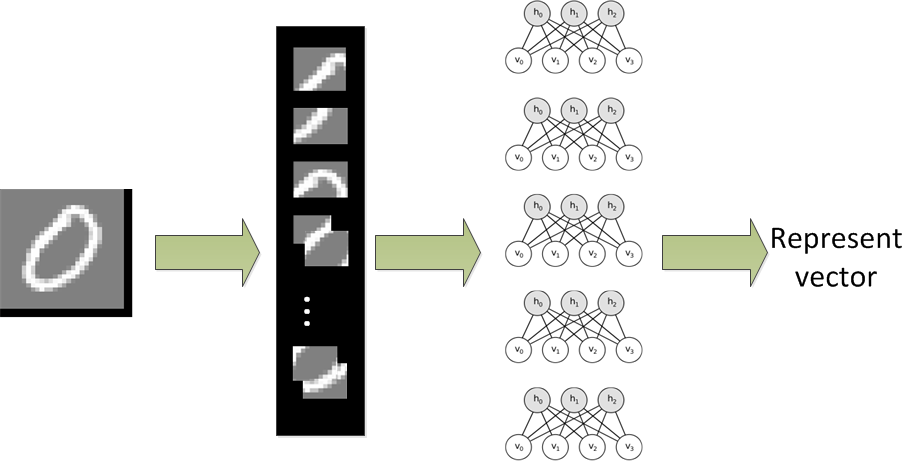
\includegraphics[scale = .5]{fig/RBM_encoder.png}\\
  \caption{Use free energy of RBMs as the encoder}
\end{figure}

 Overall, no matter the weighted Euclidean Distance or the RBM encoder with free energy, they are trying to find the proper metric to evaluate the similarity for images. SIFT can detect the same objects in two images and get rid of the affects of rotation, scaling and lighting condition \cite{lowe1999object}. However SIFT can only detect identical objects in the two images. When the two objects are not that similar, like the handwritten digital numbers written by different people, SIFT still can do nothing. Still there are a lot of researchers that are focusing on how to encoding the image effectively. Encoding the image with the centroids is still a challenge work and can be done in future works. 
\newpage
\section{Conclusion}
 This TSP has mainly cover three parts of work:
\begin{itemize}
  \item In Section \ref{sec:intro}, some concepts and the kernel based image filtering technique are introduced. The kernel based image process method is the most important technique in image recognition which is widely used in feature extraction. Kernels are often used in convolutional neural network which can be implemented very fast with the help of GPU. Therefore, the large convolutional neural network is the first choice for large real world image learning task. 
  \item In Section \ref{dl}, the deep learning method is introduced. Deep learning is the state-of-the-art and the most popular model for image recognition. It shows great power on both learning the features and image representation. Deep learning uses the stacked RBM to learning the hierarchical feature representation and use the Contrastive Divergence strategy to training the model in an unsupervised way. This feature learning idea has given inspiration to many other unsupervised feature extract methods as well as the method proposed in Section \ref{km}.
  \item In the Section \ref{km}, the kmeans based feature extract method is proposed. Inspired by the unsupervised feature extraction idea in Deep learning, I try to use kmeans to find the templates as the features for image representation. The patch combination can be the novel part of this method which combines the centroids in different location to generate the "super patch". After patch combination, the unsupervised and supervised patch ranking methods are used to eliminate the sparse, redundant and irrelevant centriods. Finally the encoding methods is introduced.
\end{itemize}

In the kmeans based feature representation method, there are less hyperparemeters so that the background knowledge becomes less important. Still there are many challenges for this method: 
\begin{itemize}
  \item In patch ranking, even though, the bad centroids and irrelevant ones are ranked low, it is still unknow for us to know what is the optimal number of features get for learning the specific problem without the help of learning curve. Thus there are a lot of work to determine the optimal number of features for this method. In my future work, some score may be used to evaluate the centroids.
  \item There is still no good solution for the encoding problem as its complexity. There are too many variables that need to be considered and still many work for me to find the best metric for the similarity measurement.
\end{itemize}
In the next few terms, all these problems above should be the main work for me and hopefully, with the supervision of Dr. Charles Ling, I can find some solutions for them and improve this method. 
 %\\
In K-means algorithm, the performance of the algorithm is mainly determined by the parameter K, which denotes the number of cluster. However, in most of the situation, it is not possible to determine a proper K. For object recognition, it could be a challenge for human to determine K for the algorithm, even though, human can distinguish objects by some features, such as color, shape, texture, etc. Many works have been done to heuristically determine the number of cluster automatically. Ray et.al \cite{ray1999determination} proposed a method that starts K from 2 to $K_{max}$, which is defined prior as the upper limit for K. Figueiredo et.al. \cite{figueiredo2002unsupervised} estimated K with minimum message length (MML) criteria and Gaussian mixture model. These methods try to learn the data distribution naturally without much human involvement, so it makes the algorithms complicate and slow. 
  \begin{figure}[ht]
    \subfloat[Original Image]{%
      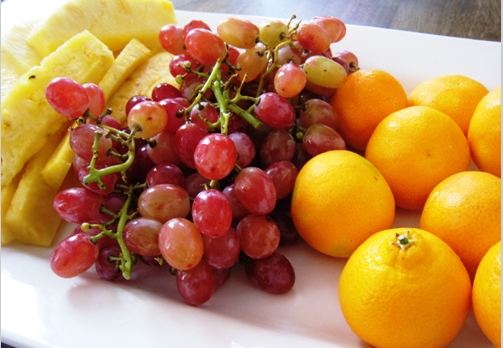
\includegraphics[width=0.45\textwidth]{fig/multdim/orig.png}
    }
    \hfill
    \subfloat[K=5]{%
       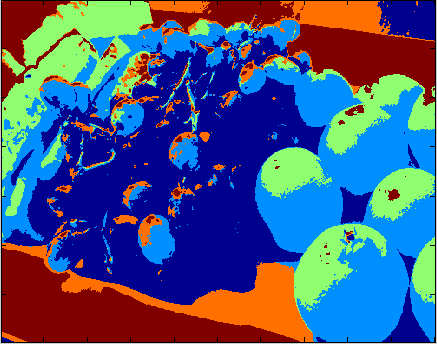
\includegraphics[width=0.45\textwidth]{fig/multdim/k5.png}
    }\\
    \subfloat[K=6]{%
      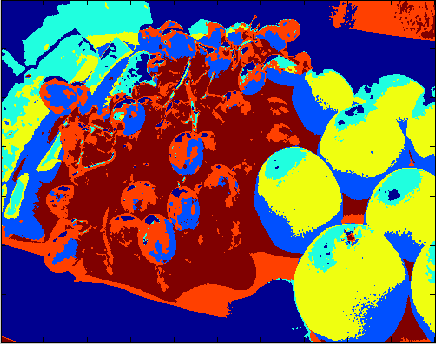
\includegraphics[width=0.45\textwidth]{fig/multdim/k6.png}
    }
    \hfill
    \subfloat[K=10]{%
       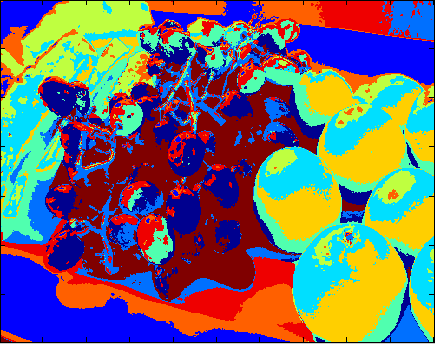
\includegraphics[width=0.45\textwidth]{fig/multdim/k10.png}
    }
    \caption{Clustering for image segmentation}
    \label{fig:cluster seg}
  \end{figure}
  
Normally smaller data can be better clustered while large volume data or data with high dimension could be a hard task for any clustering algorithm. In object recognition, our human classify objects mainly by their shapes and colors. Human have many prior knowledge that can teach the algorithm to use and this could make it simple and fast. Suppose we have to group the two-dimensional dataset in \figref{fig:multidim}.

\begin{figure}[ht]
  \centering
  % Requires \usepackage{graphicx}
  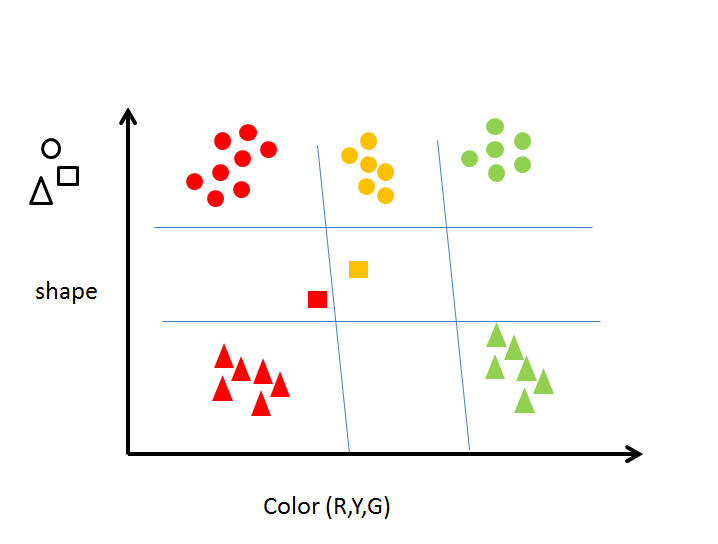
\includegraphics[width=0.7\textwidth]{fig/multdim/example.png}\\
  \caption{How multi-dimensional clustering works}
  \label{fig:multidim}
\end{figure}

 %  
  \begin{figure}[ht]
    \subfloat[Original Image]{%
      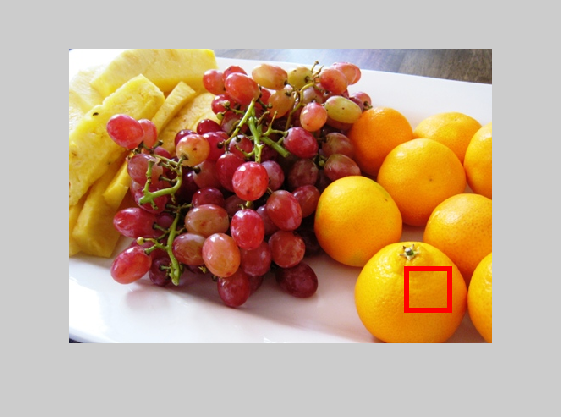
\includegraphics[width=0.45\textwidth]{fig/imagextend/orig.png}
    }
    \hfill
    \subfloat[Distance Map]{%
       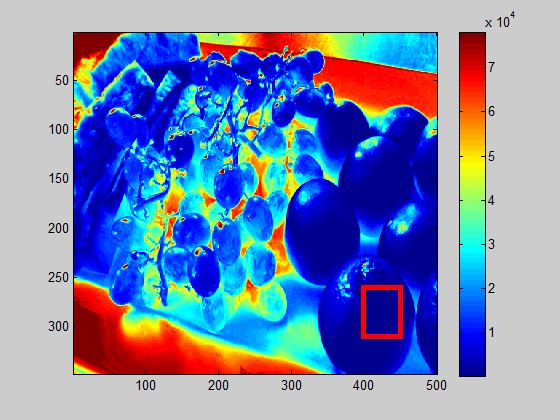
\includegraphics[width=0.45\textwidth]{fig/imagextend/distmap.png}
    }\\
    \subfloat[0.8]{%
      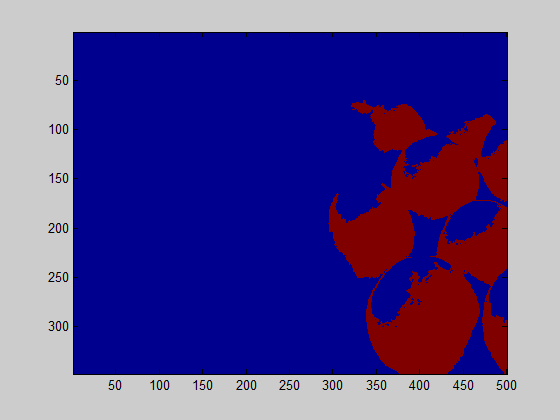
\includegraphics[width=0.45\textwidth]{fig/imagextend/8thre.png}
    }
    \hfill
    \subfloat[1.0]{%
       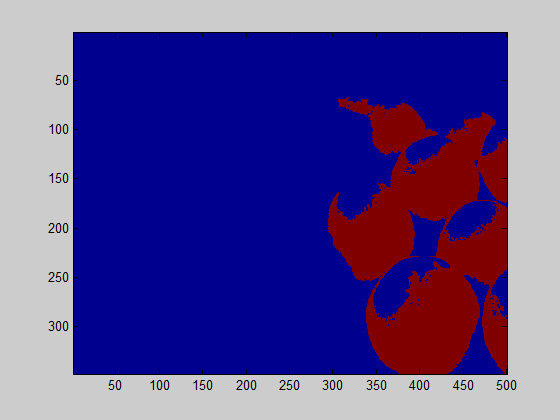
\includegraphics[width=0.45\textwidth]{fig/imagextend/1thre.png}
    }  \\
     \subfloat[1.5 ]{%
      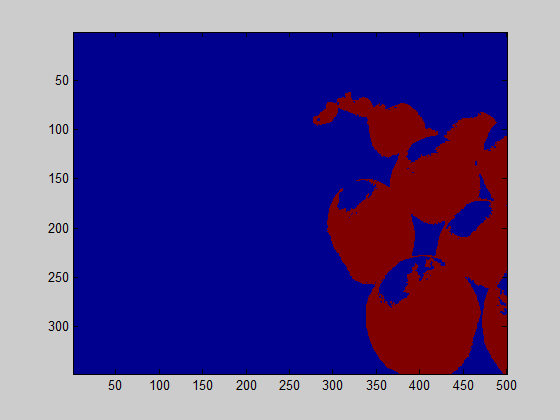
\includegraphics[width=0.45\textwidth]{fig/imagextend/15thre.png}
    }
    \hfill
    \subfloat[2]{%
       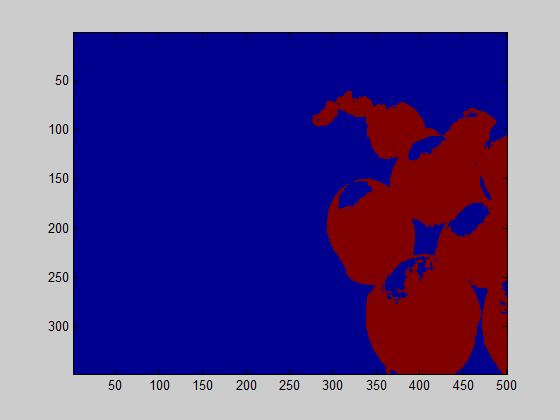
\includegraphics[width=0.45\textwidth]{fig/imagextend/2thre.png}
    }
    \caption{Clustering for image segmentation}
    \label{fig:extendthr}
  \end{figure}
 %\begin{table}
  \centering
  \begin{tabular}{|c|c|c|c|c|c|c|}
     \hline
     % after \\: \hline or \cline{col1-col2} \cline{col3-col4} ...
     method &   Time   &   Scale    &  Rotation   & Blur    &   Illumination   &   Affine\\
     \hline
    Sift   &   common  &  best    &   best     &  common  &   common   &    good\\
    \hline
    PCA-sift  &  good  &    good   &   good   &   best   &   good    &    best\\
    \hline
    Surf    &  best   &    common  &  common   &  good   &    best     &    good\\
     \hline
   \end{tabular}
  \caption{XX}
\end{table}


\newpage

\bibliographystyle{abbrv}
\bibliography{research}

%\newpage
%\appendix
%\section*{Appendix}
%\subsection{cool}

%\renewcommand{\appendixname}{Appendix~\Alph{section}}

   % \section{Some Patch Combination Results}


\end{document}
